\documentclass[expologarit]{subfiles}
\begin{document}
\begin{center}
\color{violet} \kml សិក្សាអនុគមន៍ទម្រង់ $y=f(x)=\frac{ax^2+bx+c}{px+q}$
\end{center}
{\color{violet}\kml លំហាត់ទី១} គេមានអនុគមន៍ $f$ កំណត់លើ $\mathbb{R}-\{2\}$ ដោយ $f(x)=\frac{x^2-x-1}{x-2}$ ។\\ យើងតាង $C$ ជាក្រាបរបស់វាលើតម្រុយអរតូណរម៉ាល់$\left(0,\overrightarrow{i},\overrightarrow{j}\right)$។
\begin{enumerate}[1]
\item សិក្សាលីមីតនៃអនុគមន៍ $f$ ត្រង់ $-\infty$ និងត្រង់ $+\infty$ ។
\item សិក្សាអថេរភាព និងសង់តារាងអថេរភាពនៃអនុគមន៍ $f$ ។
\item \begin{enumerate}[a]
\item រកចំនួនពិត $a,b,c$ ដែលគ្រប់ $x\neq 2;\ \ \ f(x)=ax+b+\frac{c}{x-2}$ ។
\item គេតាង $\mathrm{d}$ ដែលមានសមីការ $y=x+1$។ បង្ហាញថា $d$ ជាអាស៊ីមតូតនៃ $C$ ត្រង់ $+\infty$ និង $-\infty$។ 
\\ សិក្សាទីតាំងនៃក្រាប $C$ ធៀបនឹងបន្ទាត់ $\mathrm{d}$ ។
\item សង់ក្រាប $C$ និង បន្ទាត់ $d$ ។
\end{enumerate}
\end{enumerate}
\begin{center}
\color{violet}\kml ដំណោះស្រាយ
\end{center}
\begin{enumerate}[1]
\item សិក្សាលីមីតនៃអនុគមន៍ $f$ ត្រង់ $-\infty$ និងត្រង់ $+\infty$ 
\begin{flalign*}
&\lim_{x\to -\infty}f(x)=\lim_{x\to -\infty}\frac{x^2-x-1}{x-2}=\lim_{x\to -\infty}\frac{x^2\left(1-\dfrac{1}{x}-\dfrac{1}{x^2}\right)}{x\left(1-\dfrac{2}{x}\right)}=-\infty\frac{\left(1-0-0\right)}{1-0}=-\infty&\\
& \text{ដូចនេះ} \ \fbox{$\lim_{x\to -\infty}f(x)=-\infty$}&
\end{flalign*}
\begin{flalign*}
&\lim_{x\to +\infty}f(x)=\lim_{x\to +\infty}\frac{x^2-x-1}{x-2}=\lim_{x\to +\infty}\frac{x^2\left(1-\dfrac{1}{x}-\dfrac{1}{x^2}\right)}{x\left(1-\dfrac{2}{x}\right)}=+\infty\frac{\left(1-0-0\right)}{1-0}=+\infty &\\
& \text{ដូចនេះ} \ \fbox{$\lim_{x\to +\infty}f(x)=+\infty$}&
\end{flalign*}
\newpage 
\item សិក្សាអថេរភាព និងសង់តារាងអថេរភាពនៃអនុគមន៍ $f$ 
\begin{itemize}
\item ដេរីវេ
\begin{flalign*}
f'(x)=\left(\frac{x^2-x-1}{x-2}\right)' &=\frac{\left( x^2-x-1\right)'(x-2)-(x-2)'\left(x^2-x-1\right)}{(x-2)^2}&\\
										&=\frac{(2x-1)(x-2)-\left(x^2-x-1\right)}{(x-2)^2}\\
				&						=\frac{2x^2-4x-x+2-x^2+x+1}{(x-2)^2}=\frac{x^2-4x+3}{(x-2)^2}&
\end{flalign*}
$f'(x)=0\quad \Leftrightarrow \ x^2-4x+3=0\quad $ មានឫស $x_1=1;\ \ x_2=3$
\item តារាសញ្ញាដេរីវេ $f'(x)$
\\[0.2cm]
\begin{tikzpicture}
   \tkzTabInit[lw=1,lgt=1,espcl=1.5]{$x$ / 0.75 , $f'(x)$ / 1}{$\ \ -\infty$ , $1$,$2$,$3$, $+\infty\ \ $}
   \tkzTabLine{, +, z, - ,d,-, z,+ }
\end{tikzpicture}
\item $f'(x)>0$ ឬ អនុគមន៍ $f$ កើន ពេល $x\in\left(-\infty ,1\right)\cup\left(3,+\infty\right)$
\item $f'(x)<0$ ឬ អនុគមន៍ $f$ ចុះ ពេល $x\in\left(1,2\right)\cup\left(2,3\right)$
\item បរមាធៀប 
\begin{itemize}
\item ត្រង់ $x=1;\ f'(x)=0$ ហើយប្តូរសញ្ញាពី $+$ ទៅ $-$ \\[0.25cm]
គេបាន $f$ មានអតិបរមាធៀបមួយ គឺ $f(1)=\frac{1^2-1-1}{1-2}=1$
\item ត្រង់ $x=3;\ f'(x)=0$ ហើយប្តូរសញ្ញាពី $-$ ទៅ $+$\\[0.25cm] គេបាន $f$ មានអប្បបរមាធៀបមួយ គឺ $f(3)=\frac{3^2-3-1}{3-2}=5$
\end{itemize}
\newpage
\item តារាងអថេរភាពនៃ $f$\\[0.2cm]
\begin{tikzpicture}
   \tkzTabInit[lw=1,lgt=1,espcl=1.5]{$x$ / 0.75 , $f'(x)$ / 1, $f(x)$/2}{$\ \ -\infty$ , $1$,$2$,$3$, $+\infty\ \ $}
   \tkzTabLine{, +, z, - ,d,-, z,+ }
   \tkzTabVar{-/ $ -\infty$, +/$1$, -D+/ $-\infty$ /$+\infty$, -/ $5$ , +/ $+\infty$}
\end{tikzpicture}
\end{itemize}
\item \begin{enumerate}[a]
\item រកចំនួនពិត $a,b,c$ ដែលគ្រប់ $x\neq 2;\ \ \ f(x)=ax+b+\frac{c}{x-2}$ 
\begin{flalign*}
f(x)=ax+b+\frac{c}{x-2}\quad &\Leftrightarrow\ \frac{x^2-x-1}{x-2} \quad\quad\quad \quad  =ax+b+\frac{c}{x-2}&\\
											&\Leftrightarrow\ \frac{(x-2)(x+1)+1}{x-2} \quad =ax+b+\frac{c}{x-2}&\\
											&\Leftrightarrow\ x+1+\frac{1}{x-2} \quad \ \ \ \quad =ax+b+\frac{c}{x-2}
\end{flalign*}
ដោយផ្ទឹមមេគុណ យើងបាន \quad \fbox{$a=1;\ b=1;\ c=1$}
\item  បង្ហាញថា $d:\ y=x+1$ ជាអាស៊ីមតូតនៃ $C$ ត្រង់ $+\infty$ និង $-\infty$\\[0.25cm]
ដោយ $\lim_{x\to \pm \infty}[f(x)-(x+1)]=\lim_{x\to \pm \infty}\left[ x+1+\frac{1}{x-2}-(x+1)\right]=\lim_{x\to\pm\infty}\frac{1}{x-2}=0 $\\[0.25cm]
ដូចនេះ \ \fbox{ បន្ទាត់ $d:\ y=x+1$ ជាអាស៊ីមតូតនៃ $C$ }\\[0.25cm]
សិក្សាទីតាំងនៃក្រាប $C$ ធៀបនឹងបន្ទាត់ $\mathrm{d}$ 
\\ $C:\ y=x+1+\frac{1}{x-2}\quad ;\ d:\ y=x+1\\[0.25cm]  \Rightarrow\ y_c-y_d=x+1+\frac{1}{x-2}-(x+1)=\frac{1}{x-2}$\\
\begin{itemize}
\item $y_c-y_d> 0 \quad \Leftrightarrow   \frac{1}{x-2}>0\quad\Leftrightarrow x-2>0\quad \Leftrightarrow\ x>2$\\[0.25cm]
ដូចនេះ \ \fbox{ $(c)$ ស្ថិតនៅលើបន្ទាត់ $(d)$ ពេល $x>2$ }

\newpage 
\item $y_c-y_d< 0 \quad \Leftrightarrow  \frac{1}{x-2}<0\quad\Leftrightarrow  x-2<0\quad \Leftrightarrow\ x<2$\\[0.25cm]
ដូចនេះ \ \fbox{ $(c)$ ស្ថិតនៅក្រោមបន្ទាត់ $(d)$ ពេល $x<2$ }
\end{itemize} 
\item សង់ក្រាប $C$ និង បន្ទាត់ $d$ \\
$(C)\cap (x'ox)$\ គឺ $y=o\\[0.25cm] \Leftrightarrow\ x^2-x-1=0\quad \Delta =b^2-4ac=(-1)^2-4(1)(-1)=5 $ មានឫស $x=\frac{1\pm\sqrt{5}}{2}$ \\ គេបាន $x=1.62\quad , \quad x=-0.62$  \\[0.25cm]
$(C)\cap (y'oy) \Leftrightarrow x=0\quad\Rightarrow\ y=\frac{0^2-0-1}{0-2}=\frac{1}{2} $
\begin{center}
\definecolor{qqwuqq}{rgb}{0.,0.39215686274509803,0.}
\begin{tikzpicture}[scale=0.8]
\draw(0,9)node{$
\begin{array}{l}
(d):\ y=x+1\\
\begin{tabular}{c|cc}
$x$&$0$&$-1$\\
\hline 
$y$&$1$&$0$
\end{tabular}
\end{array}
$};
\begin{axis}[
x=1.0cm,y=1.0cm,
axis lines=middle,
xmin=-3,
xmax=7.5,
ymin=-3,
ymax=8,
xlabel=$x$,ylabel=$y$,
xtick={-3.0,-2.0,...,6.0},
ytick={-3.0,-2.0,...,7.0},]
\draw[line width=1.pt,color=qqwuqq,smooth,samples=140,domain=-2.9:5.8] plot(\x,{((\x)^(2)-(\x)-1)/((\x)-2.0)});
\draw [line width=1.pt,domain=-3.:6.] plot(\x,{(--1.--1.*\x)/1.});
\draw(0,1)--(5,6)node[sloped, very near end,below]{$(d):\ y=x+1$};
\draw(4,7.5)node[color=qqwuqq, left=1cm]{$(c)$};
\draw(2.5,-2.5)node[color=qqwuqq]{$x=2$};
\draw [dashed](3,0)--(3,5)node{$\bullet$}--(0,5); 
\draw [dashed](1,0)--(1,1)node{$\bullet$}--(0,1); 
\draw [dashed](1.62,0)--(1.62,0)node{$\bullet$}--(-0.62,0)node{$\bullet$}; 
\draw[dashed](0,3)--(2,3)node{$\bullet$};
\draw (0,0.5)node{$\bullet$};
\end{axis}
\end{tikzpicture}
\end{center}
\end{enumerate}
\end{enumerate}
\newpage 
\begin{center}
\color{violet} {\kml លំហាត់ទី២}
\end{center}
គេមានអនុគមន៍ $f$ ដែល $f(x)=\frac{x^2-x-3}{x+1}$  និង គេតាងដោយ $(C)$  ក្រាបនៃអនុគមន៍ $f$ ។
			\begin{enumerate}[k]
			\item រកដែនកំណត់នៃអនុគន៍ $f$ ។
			\item បង្ហាញថា  $f(x)=x-2-\frac{1}{x+1}$ ។
			\item បង្ហាញថាបន្ទាត់ដែលមានសមីការ  $y=x-2$ ជាអាស៊ីមតូតទ្រេតនៃក្រាប $(C)$ ។
			\item សិក្សាអថេរភាព និងសង់ក្រាបនៃ $f$ ។
			\end{enumerate}
			
			\begin{center}
			\color{violet} \kml ដំណោះស្រាយ
			\end{center}
				\begin{enumerate}[k]
			\item រកដែនកំណត់នៃអនុគន៍ $f$ 
			\\[0.2cm] ដោយ \ $f(x)=\frac{x^2-x-3}{x+1}$  ;\quad  $f(x)$ មានន័យលុះត្រាតែ $x+1\neq 0\quad \Leftrightarrow \ x\neq -1$\\[0.2cm]
			ដូចនេះ \ \fbox{ដែនកំណត់នៃអនុគមន៍ $f$ គឺ $D_f=\mathbb{R}-\{-1\}$}

			\item បង្ហាញថា  $f(x)=x-2-\frac{1}{x+1}$ 
			\begin{flalign*}
		&\text{ដោយ}\quad 	x-2-\frac{1}{x+1}=\frac{(x-2)(x+1)-1}{x+1}=\frac{x^2+x-2x-2-1}{x+1}=\frac{x^2-x-3}{x+1}=f(x)&
			\end{flalign*}
			ដូចនេះ \ \fbox{$f(x)=x-2-\frac{1}{x+1}$}
			\item បង្ហាញថាបន្ទាត់ដែលមានសមីការ  $y=x-2$ ជាអាស៊ីមតូតទ្រេតនៃក្រាប $(C)$ 
			\begin{flalign*}
		&	\text{ដោយ} \ \lim_{x\to \pm \infty}\left[f(x)-(x-2)\right]=\lim_{x\to \pm\infty}\left[x-2-\frac{1}{x+1}-(x-2)\right]= \lim_{x\to \pm\infty }\frac{-1}{x+1}=0&
			\end{flalign*}
			ដូចនេះ \ \fbox{បន្ទាត់ $y=x-2$ ជាអាស៊ីមតូតទ្រេតនៃក្រាប$C$}
			\newpage 
			\item សិក្សាអថេរភាព និងសង់ក្រាបនៃ $f$ 
			\begin{itemize}
			\item ដេរីវេ
			\begin{flalign*}
				f'(x)&=\left(\frac{x^2-x-3}{x+1}\right)' =\frac{\left(x^2-x-3\right)'(x+1)-(x+1)'\left(x^2-x-3\right)}{(x+1)^2}
				&\\
				&=\frac{(2x-1)(x+1)-\left(x^2-x-3\right)}{(x+1)^2} &\\ &=\frac{2x^2+2x-x-1-x^2+x+3}{(x+1)^2}=\frac{x^2+2x+2}{(x+1)^2};\\ 
				f'(x)&=0\quad \Leftrightarrow \ x^2+2x+2=0 \quad \Delta =b^2-4ac=4-4(1)2=-4<0 \\
			f'(x)	& \text{មានសញ្ញាតាមមេគុណ\ $a$}
			\end{flalign*}
\end{itemize}

\begin{itemize} 
\item តារាងសញ្ញា $f'(x)$		
\\[0.2cm]
\begin{tikzpicture}
   \tkzTabInit[lw=1,lgt=1,espcl=2]{$x$ / 0.75 , $f'(x)$ / 1}{$-\infty$ , $-1$, $+\infty $}
   \tkzTabLine{,+,d,+, }
\end{tikzpicture}	
\\[0.25cm]
$f'(x)>0$ ឬ អនុគមន៍ $f$ កើន ពេល $x\in\left(-\infty,-1\right)\cup\left(-1,+\infty\right) $
\item តារាងអថេរភាពនៃ $f$
\\[0.2cm]
\begin{tikzpicture}
   \tkzTabInit[lw=1,lgt=1,espcl=3]{$x$ / 0.75 , $f'(x)$ / 1, $f(x)$/1.5}{$\ \ -\infty$ ,$-1$, $+\infty\ \ $}
   \tkzTabLine{, +, d, + , }
   \tkzTabVar{-/ $-\infty$,  +D-/ $+\infty$ /$-\infty$, +/ $+\infty$ }
\end{tikzpicture}
\end{itemize}
\begin{itemize}
\item សង់ក្រាប
\begin{itemize}
\item $C\cap (y'oy)$\ គឺ\ $x=0;\ \Rightarrow\ y=\frac{0^2-0-3}{0+1}=-3$
\item $C\cap (x'ox)$\ គឺ \ $y=0\ \Rightarrow\ x^2-x-3=0\\[0.25cm]
 \Delta =b^2-4ac=(-1)^2-4(1)(-3)=13\ \Rightarrow\ x=\frac{1\pm\sqrt{13}}{2};\ x=2.3,\ x=-1.3$
\end{itemize}
\begin{center}
\definecolor{qqwuqq}{rgb}{0.,0.39215686274509803,0.}
\begin{tikzpicture}[x=1cm,y=1cm]
\begin{axis}[
x=0.91cm,y=0.91cm,
axis lines=middle,
xmin=-6,
xmax=7,
ymin=-8,
ymax=5.5,
xlabel=$x$,ylabel=$y$,
xtick={-6.0,-5.0,...,6.0},
ytick={-6.0,-5,-4,...,6},]
\draw[line width=1.pt,color=qqwuqq,smooth,samples=150,domain=-5:5.9] plot(\x,{((\x)^(2)-(\x)-3)/((\x)+1.0)});
\draw [line width=1.pt,domain=-5.:5.9] plot(\x,{\x-2});
\draw(0,-2)--(5,3)node[sloped, near end, above]{$(d):\ y=x-2$};
\draw(-2,7.5)node[color=qqwuqq]{$(c)$};
\draw(-1,0)--(-1,-6)node[color=qqwuqq,sloped,very near end,below]{$x=-1$};
\draw(-1.3,0)node{$\bullet$};
\draw(2.3,0)node{$\bullet$};
\draw(0,-3)node{$\bullet$};
\draw(0,-2)node{$\bullet$};
\draw(2,0)node{$\bullet$};
%\draw [dashed](3,0)--(3,5)node{$\bullet$}--(0,5); 
%\draw [dashed](1,0)--(1,1)node{$\bullet$}--(0,1); 
\draw(-4,4)node{$
\begin{array}{l}
(d):\ y=x-2\\
\begin{tabular}{c|cc}
$x$&$0$&$2$\\
\hline 
$y$&$-2$&$0$
\end{tabular}
\end{array}
$};
\end{axis}
\end{tikzpicture}
\end{center}
\end{itemize} 
			\end{enumerate}	
			
			\newpage 
			\begin{center}
		\color{violet}	\kml លំហាត់ទី៣
			\end{center}
	គេមានអនុគមន៍ $f(x)=\frac{(x+2)(x-2)}{(1-x)}$ ។
\begin{enumerate}[k]
\item រកដែនកំណត់ $f(x)$ ។
\item បង្ហាញថា $f(x)=-x-1+\frac{3}{x-1}$ ។
\item សិក្សាអថេរភាពនិង សង់ក្រាប $C$ នៃអនុគមន៍ $f(x)=\frac{(x+2)(x-2)}{(1-x)}$ ។
\end{enumerate}

\begin{center}
\color{violet} \kml ដំណោះស្រាយ
\end{center}
\begin{enumerate}[k]
\item រកដែនកំណត់ $f(x)$ \quad ; $f(x)=\frac{(x+2)(x-2)}{1-x}$
\begin{flalign*}
& f(x)\  \text{មានន័យលុះត្រាតែ}\  1-x\neq 0\quad \Leftrightarrow \ x\neq 1& \\[0.25cm]
&\text{ ដូចនេះ}  \ \fbox{ដែនកំណត់នៃអនុគមន៍ $f$ គឺ $D_f=\mathbb{R}-\{1\}$} &
\end{flalign*}
\item បង្ហាញថា $f(x)=-x-1+\frac{3}{x-1}$ 
\begin{flalign*}
\text{ដោយ}\ -x-1+\frac{3}{x-1}=\frac{(-x-1)(x-1)+3}{x-1}&=\frac{-x^2+x-x+1+3}{-(1-x)}&\\
&=\frac{-\left(x^2-4\right)}{-(1-x)}\\
&=\frac{(x+2)(x-2)}{1-x}\\
&=f(x)&
\end{flalign*}
ដូចនេះ\ \fbox{$f(x)=-x-1+\frac{3}{x-1}$}
\newpage
\item សិក្សាអថេរភាពនិង សង់ក្រាប $C$ 
\begin{itemize}
\item ដេរីវេ
\begin{flalign*}
f'(x)&=\left(\frac{(x+2)(x-2)}{1-x}\right)' =\left(\frac{x^2-4}{1-x}\right)'=\frac{\left(x^2-4\right)'(1-x)-(1-x)'\left(x^2-4\right)}{(1-x)^2} &\\
&=\frac{2x(1-x)+\left(x^2-4\right)}{(1-x)^2}=\frac{2x-2x^2+x^2-4}{(1-x)^2}=\frac{-x^2+2x-4}{(1-x)^2}&\\
f'(x)&=0\quad\Leftrightarrow\ -x^2+2x-4=0\\[0.25cm]
\Delta &=b^2-4ac=(2)^2-4(-1)(-4)=4-16=-12<0&\\
\text{គេបាន} &  f'(x) \ \text{មានសញ្ញាដូចមេគុណ $a$} 
\end{flalign*}

\end{itemize}
\begin{itemize}
\item តារាងសញ្ញា $f'(x)$		
\\[0.2cm]
\begin{tikzpicture}
   \tkzTabInit[lw=1,lgt=1,espcl=1.5]{$x$ /0.75 , $f'(x)$ / 1}{$\ \ -\infty$ , $1$, $+\infty\ \ $}
   \tkzTabLine{,-,d,-, }
\end{tikzpicture}	\\[0.25cm]
$f'(x)<0$ ឬអនុគមន៍ $f$ ចុះ ពេល $x\in\left(-\infty ,1\right)\cup\left(1,+\infty\right)$
\item លីមីត
\begin{flalign*}
&\lim_{x\to \pm\infty}f(x)=\lim_{x\to \pm\infty}\frac{x^2-4}{1-x}=\mp \infty &\\
& \lim_{x\to 1}f(x)=\lim_{x\to 1}\frac{x^2-4}{1-x}=\pm\infty&
\end{flalign*}

\item តារាងអថេរភាពនៃ $f$
\\[0.2cm]
\begin{tikzpicture}
   \tkzTabInit[lw=1,lgt=1,espcl=3]{$x$ / 0.75 , $f'(x)$ / 1, $f(x)$/1.5}{$\ \ -\infty$ ,$1$, $+\infty\ \ $}
   \tkzTabLine{, -, d, - , }
   \tkzTabVar{+/ $+\infty$,  -D+/ $-\infty$ /$+\infty$, -/ $-\infty$ }
\end{tikzpicture}
\end{itemize}
\begin{itemize}
\newpage
\item សង់ក្រាប 
\begin{itemize}
\item  ក្រាប$(c)$ កាត់អ័ក្សអរដោនេ ពេល$x=0\quad\Rightarrow y=f(0)=\frac{(0+2)(0-2)}{1-0}=-4$
\item ក្រាប $(c)$ កាត់អ័ក្សអាប់ស៊ីស ពេល $y=0\ \Leftrightarrow \ 0=\frac{(x+2)(x-2)}{(1-x)}\ \Leftrightarrow \ x=-2;\ x=2$
\end{itemize}
\begin{center}
\definecolor{qqwuqq}{rgb}{0.,0.39215686274509803,0.}
\begin{tikzpicture}[x=1cm,y=1cm]
\draw(1,12.5)node{$
\begin{array}{l}
(d):\ y=-x-1\\
\begin{tabular}{c|cc}
$x$&$0$&$-1$\\
\hline 
$y$&$-1$&$0$
\end{tabular}
\end{array}
$};
\begin{axis}[
x=0.7cm,y=0.7cm,
axis lines=middle,
xmin=-8.5,
xmax=9,
ymin=-9,
ymax=8.5,
xlabel=$x$,ylabel=$y$,
xtick={-8,-6.0,...,8},
ytick={-8,-6.0,...,6.0},]
\draw[line width=1.pt,color=qqwuqq,smooth,samples=180,domain=-8:8] plot(\x,{((\x)^(2)-4)/(1-\x)});
\draw [line width=1.pt,domain=-8.:8] plot(\x,{-\x-1});
\draw(0,-1)--(-8,7)node[sloped, near end,above]{$(d):\ y=-x-1$};
\draw(2,5)node[color=qqwuqq]{$(c)$};
\draw (-2,0)node{$\bullet$}--(2,0)node{$\bullet$};
\draw (0,-4)node{$\bullet$};
\draw(1,0)--(1,-8)node[color=qqwuqq,sloped,very near end, above]{$x=1$};
\draw [dashed](1,0)--(1,-2)node{$\bullet$}--(0,-2); 
\end{axis}
\end{tikzpicture}
\end{center}
\end{itemize}
\end{enumerate}
\newpage 
\begin{center}
\color{violet} \kml លំហាត់ទី៤
\end{center}
គេឲ្យអនុគមន៍ $f$ កំណត់ដោយ $f(x)=\frac{x^2+x+4}{x+1}$ ហើយមានក្រាប $C$ ។
\begin{enumerate}[m]
\item រកដែនកំណត់ និង សិក្សាសញ្ញាដេរីវេ $f'(x)$ នៃអនុគមន៍ $f$ ។
\item សរសេរសមីការអាស៊ីមតូតឈរ និង អាស៊ីមតូតទ្រេតនៃក្រាប $C$ ។
\item សង់តារាងអថេរភាព អាស៊ីមតូត និង ក្រាប $C$ នៃអនុគមន៍ $f$ ។
\end{enumerate}
\begin{center}
\color{violet} \kml ដំណោះស្រាយ
\end{center}
\begin{enumerate}[m]
\item រកដែនកំណត់  \\
យើងមាន  $f(x)=\frac{x^2+x+4}{x+1}$  
\begin{itemize}
\item $f(x)$ មានន័យលុះត្រាតែ $x+1\neq 0\quad\Rightarrow \ x\neq -1$
\end{itemize}
ដូចនេះ \fbox{ដែនកំណត់នៃ $f$ គឺ $D_f=\mathbb{R}-\{-1\}$ }\\[0.25cm]
សិក្សាសញ្ញាដេរីវេ $f'(x)$ នៃអនុគមន៍ $f$
\begin{flalign*}
f'(x)&=\left(\frac{x^2+x+4}{x+1}\right)'=\frac{\left(x^2+x+4\right)'(x+1)-(x+1)'\left(x^2+x+4\right)}{(x+1)^2} &\\
&=\frac{(2x+1)(x+1)-x^2-x-4}{(x+1)^2}=\frac{2x^2+2x+x+1-x^2-x-4}{(x+1)^2}\\
&=\frac{x^2+2x-3}{(x+1)^2}
\end{flalign*}
ដោយ $(x+1)^2>0\quad \forall x\in D_f$ គេបាន
\begin{itemize}
\item  $f'(x)$ មានសញ្ញាដូចភាគយក $x^2+2x-3$
\item 
$f'(x)=0\quad\Leftrightarrow\quad x^2+2x-3=0\quad $ មានឬស $x_1=1,\ x_2=-3$
\end{itemize}
តារាសញ្ញាដេរីវេ $f'(x)$
\\[0.2cm]
\begin{tikzpicture}
   \tkzTabInit[lw=1,lgt=1,espcl=1.5]{$x$ / 0.75 , $f'(x)$ / 1}{$\ \ -\infty$ , $-3$,$-1$,$1$, $+\infty\ \ $}
   \tkzTabLine{, +, z, - ,d,-, z,+ }
\end{tikzpicture}
\begin{itemize}
\item $f'(x)>0$ ឬ អនុគមន៍ $f$ កើន ពេល $x\in (-\infty ,-3)\cup (1,+\infty)$
\item $f'(x)<0$ ឬ អនុគមន៍ $f$ ចុះ ពេល $x\in (-3,-1)\cup (-1,1)$
\item ត្រង់ $x=-3;\ f'(x)=0$ ហើយប្តូរសញ្ញាពី $+$ ទៅ $-$ \\[0.25cm]
គេបាន $f$ មានអតិបរមាធៀបមួយ គឺ $f(-3)=\frac{9-3+4}{-3+1}=-5$
\item ត្រង់ $x=1;\ f'(x)=0$ ហើយប្តូរសញ្ញាពី $-$ ទៅ $+$\\[0.25cm] គេបាន $f$ មានអប្បបរមាធៀបមួយ គឺ $f(1)=\frac{1^2+1+4}{1+1}=3 $
\end{itemize}

\item សរសេរសមីការអាស៊ីមតូតឈរ និង អាស៊ីមតូតទ្រេតនៃក្រាប $C$ 
\begin{itemize}
 \item ដោយ $\lim_{x\to -1}f(x)=\lim_{x\to -1}\frac{x^2+x+4}{x+1}=\pm\infty$\\[0.25cm] ដូចនេះ \fbox{បន្ទាត់ $x=-1$ ជាសមីការអាស៊ីមតូតឈរ}
 \item $f(x)=\frac{x^2+x+4}{x+1}=x+\frac{4}{x+1}$\quad ដោយ $\lim_{x\to \pm\infty}\frac{4}{x+1}=0$\\[0.25cm]
 ដូចនេះ \fbox{បន្ទាត់ $y=x$ ជាអាស៊ីមតូតទ្រេត}
\end{itemize}
\item សង់តារាងអថេរភាព អាស៊ីមតូត និង ក្រាប $C$ នៃអនុគមន៍ $f$ \\
 តារាងអថេរភាពនៃ $f$\\[0.2cm]
\begin{tikzpicture}
   \tkzTabInit[lw=1,lgt=1,espcl=1.5]{$x$ / 0.75, $f'(x)$ / 1, $f(x)$/2}{$\ \ -\infty$ , $-3$,$-1$,$1$, $+\infty\ \ $}
   \tkzTabLine{, +, z, - ,d,-, z,+ }
   \tkzTabVar{-/ $ -\infty$, +/$-5$, -D+/ $-\infty$ /$+\infty$, -/ $3$ , +/ $+\infty$}
\end{tikzpicture}
\end{enumerate}
សង់ក្រាប$(C)$\\[0.25cm]
$(C)\cap (y'oy)\Leftrightarrow x=0\quad\Rightarrow y=\frac{0^2+0+4}{0+1}=4$
\begin{center}
\definecolor{qqwuqq}{rgb}{0.,0.39215686274509803,0.}
\begin{tikzpicture}[scale=0.8]
\draw(1,17.5)node{$
\begin{array}{l}
(d):\ y=x\\
\begin{tabular}{c|cc}
$x$&$1$&$2$\\
\hline 
$y$&$1$&$2$
\end{tabular}
\end{array}
$};
\begin{axis}[
x=1cm,y=1cm,
axis lines=middle,
xmin=-8,
xmax=7.5,
ymin=-10,
ymax=8,
xlabel=$x$,ylabel=$y$,
xtick={-8.0,-7.0,...,7.0},
ytick={-9.0,-8.0,...,7.0},]
\draw[line width=1.pt,color=qqwuqq,smooth,samples=140,domain=-8:6] plot(\x,{((\x)^(2)+(\x)+4)/((\x)+1.0)});
\draw [line width=1.pt,domain=-8:6.] plot(\x,{(\x)/1.});
\draw(1,1)--(5,5)node[sloped, very near end,below]{$(d):\ y=x$};
\draw(5,6.2)node[color=qqwuqq]{$(c)$};
\draw(-1,-5)--(-1,-3)node[color=qqwuqq,sloped,near end, above]{$x=-1$};
\draw [dashed](2,0)--(2,2)node{$\bullet$}--(0,2); 
\draw [dashed](1,0)--(1,1)node{$\bullet$}--(0,1); 
\draw [dashed](1,0)--(1,3)node{$\bullet$}--(0,3); 
\draw [dashed](-3,0)--(-3,-5)node{$\bullet$}--(0,-5); 
\draw (-1,-1)node{$\bullet$};
\draw (0,4)node{$\bullet$};
\end{axis}
\end{tikzpicture}
\end{center}
\newpage 
\begin{center}
\color{violet} \kml លំហាត់ទី៥
\end{center}
 គេមានអនុគមន៍ $f(x)=\frac{x^2+3x+6}{x+2}$  កំណត់ចំពោះគ្រប់ $x\neq -2$ និងមានខ្សែកោង $C$។
\begin{enumerate}[m]
\item គណនា  $f'(x)$។ រកតម្លៃបរមានៃ $f$។ រកសមីការអាស៊ីមតូតនៃខ្សែកោង $C$។\\ គណនាលីមីតនៃ $f$  កាលណា $x$ ខិតទៅ $+\infty,\ -\infty$។ សង់តារាងអថេរភាពនៃ $f$។
\item រកសមីការបន្ទាត់ប៉ះនឹងខ្សែកោង $C$  ត្រង់ចំណុច $x_0=1$។\\ គណនាកូអរដោនេនៃចំណុចប្រសព្វ $A$ រវាងសមីការបន្ទាត់ប៉ះនឹងអាស៊ីមតូតទ្រេតនៃខ្សែកោង $C$។
\item សង់ខ្សែកោង $C$ បន្ទាត់ប៉ះនៃខ្សែកោង $C$ និងអាស៊ីមតូត នៅក្នុងតម្រុយអរតូណរម៉ាល់តែមួយ។\\ គណនាផ្ទៃក្រទ្បាខណ្ឌដោយខ្សែកោង $C$  អ័ក្សអាប់ស៊ីស និងបន្ទាត់ $x=1,\ x=2$។
\end{enumerate}

\begin{center}
\color{violet} \kml ដំណោះស្រាយ
\end{center}
\begin{enumerate}[m]
\item គណនា  $f'(x)$\\
ដោយ $f(x)=\frac{x^2+3x+6}{x+2}$ យើងបាន 
\begin{flalign*}
f'(x)&=\left(\frac{x^2+3x+6}{x+2}\right)'=\frac{\left(x^2+3x+6\right)'\left(x+2\right)-(x+2)'\left(x^2+3x+6\right)}{\left(x+2\right)^2}&\\
&=\frac{(2x+3)(x+2)-\left(x^2+3x+6\right)}{(x+2)^2}=\frac{2x^2+4x+3x+6-x^2-3x-6}{(x+2)^2}\\
&=\frac{x^2+4x}{(x+2)^2}
\end{flalign*}
ដូចនេះ \fbox{$f'(x)=\frac{x^2+4x}{(x+2)^2}$}\\[0.25cm]
 រកតម្លៃបរមានៃ $f$\\
ដោយ $\left(x+2\right)^2> 0\quad\forall x\neq -2$\quad យើងបាន $f'(x)$ មានសញ្ញាតាមភាគយក\\
$f'(x)=0\quad \Leftrightarrow\quad x^2+4x=0\quad \Leftrightarrow\ x(x+4)=0\quad \Rightarrow x=0, x=-4$
\newpage 
តារាសញ្ញាដេរីវេ $f'(x)$
\\[0.2cm]
\begin{tikzpicture}
   \tkzTabInit[lw=1,lgt=1,espcl=1.5]{$x$ / 0.75 , $f'(x)$ / 1}{$\ \ -\infty$ , $-4$,$-2$,$0$, $+\infty\ \ $}
   \tkzTabLine{, +, z, - ,d,-, z,+ }
\end{tikzpicture}
\begin{itemize}
\item ត្រង់ $x=-4;\ f'(x)=0$ ហើយប្តូរសញ្ញាពី $+$ ទៅ $-$ 
គេបាន $f$ មានអតិបរមាធៀបមួយ គឺ \\[0.25cm] $f(-4)=\frac{16-12+6}{-4+2}=-5$
\item ត្រង់ $x=0;\ f'(x)=0$ ហើយប្តូរសញ្ញាពី $-$ ទៅ $+$  គេបាន $f$ មានអប្បបរមាធៀបមួយ គឺ \\[0.25cm] $f(0)=\frac{0+0+6}{0+2}=3$
\end{itemize}
ដូចនេះ \fbox{តម្លៃអតិបរមធៀបគឺ $-5$  តម្លៃអប្បបរមាធៀបគឺ $3$}\\[0.25cm]
 រកសមីការអាស៊ីមតូតនៃខ្សែកោង $C$
 \begin{itemize}
 \item អាស៊ីមតូតឈរ\\
 ដោយ $\lim_{x\to \pm -2}f(x)=\lim_{x\to -2}\frac{x^2+3x+6}{x+2}=\pm\infty$\\[0.25cm] ដូចនេះ \fbox{បន្ទាត់ $x=-2$ ជាអាស៊ីមតូតឈរ}
 \item អាស៊ីមតូតទ្រេត\\
 យើងមាន $f(x)=\frac{x^2+3x+6}{x+2}=x+1+\frac{4}{x+2}$\\
 ដោយ $\lim_{x\to \pm\infty}\frac{4}{x+2}=0$\\[0.25cm] ដូចនេះ \fbox{បន្ទាត់ $y=x+1$ ជាអាស៊ីមតូតទ្រេត}
 \end{itemize}
 គណនាលីមីតនៃ $f$  កាលណា $x$ ខិតទៅ $+\infty,\ -\infty$
\begin{flalign*}
\lim_{x\to +\infty}f(x)&=\lim_{x\to +\infty}\frac{x^2+3x+6}{x+2}=\lim_{x\to +\infty}\frac{x^2\left(1+\frac{3}{x}+\frac{6}{x^2}\right)}{x\left(1+\frac{2}{x}\right)}&\\
&=\lim_{x\to +\infty}\frac{x\left(1+\frac{3}{x}+\frac{6}{x^2}\right)}{1+\frac{2}{x}}=\frac{+\infty\left(1+0+0\right)}{1+0}=+\infty\\
\lim_{x\to -\infty}f(x)&=\lim_{x\to -\infty}\frac{x^2+3x+6}{x+2}=\lim_{x\to -\infty}\frac{x^2\left(1+\frac{3}{x}+\frac{6}{x^2}\right)}{x\left(1+\frac{2}{x}\right)}&\\
&=\lim_{x\to -\infty}\frac{x\left(1+\frac{3}{x}+\frac{6}{x^2}\right)}{1+\frac{2}{x}}=\frac{-\infty\left(1+0+0\right)}{1+0}=-\infty
\end{flalign*} 
 ដូចនេះ \fbox{$\lim_{x\to \pm \infty}f(x)=\pm\infty$}\\[0.25cm]
  តារាងអថេរភាពនៃ $f$\\[0.2cm]
\begin{tikzpicture}
   \tkzTabInit[lw=1,lgt=1,espcl=1.5]{$x$ / 0.75 , $f'(x)$ / 1, $f(x)$/1.5}{$\ \ -\infty$ , $-4$,$-2$,$0$, $+\infty\ \ $}
   \tkzTabLine{, +, z, - ,d,-, z,+ }
   \tkzTabVar{-/ $ -\infty$, +/$-5$, -D+/ $-\infty$ /$+\infty$, -/ $3$ , +/ $+\infty$}
\end{tikzpicture}
\item រកសមីការបន្ទាត់ប៉ះនឹងខ្សែកោង $C$  ត្រង់ចំណុច $x_0=1$\\
សមីការបន្ទាត់ប៉ះកំណត់ដោយ $y=f'(x_o)(x-x_o)+f(x_o)$\\
ដោយ បន្ទាត់ប៉ះក្រាប ត្រង់ចំណុច $x_o=1$ យើងបាន
\begin{itemize}
\item $f'(x_o)=f'(1)=\frac{1^2+4(1)}{(1+2)^2}=\frac{5}{9}$
\item $f(x_o)=f(1)=\frac{1^2+3(1)+6}{1+2}=\frac{10}{3}$
\end{itemize}
នាំឲ្យ សមីការបន្ទាត់ប៉ះគឺ $y=\tfrac{5}{9}\left(x-1\right)+\tfrac{10}{3}=\tfrac{5}{9}x+\tfrac{25}{9}$\\[0.25cm]
ដូចនេះ \fbox{សមីការបន្ទាត់ប៉ះគឺ $y=\tfrac{5}{9}x+\tfrac{25}{9}$}\\
គណនាកូអរដោនេនៃចំណុចប្រសព្វ $A$ រវាងសមីការបន្ទាត់ប៉ះនឹងអាស៊ីមតូតទ្រេតនៃខ្សែកោង $C$\\
 ដោយ អាស៊ីមតូតទ្រេតគឺ $d:\ y=x+1 $ ;\quad  បន្ទាត់ប៉ះគឺ $L:\  y= \tfrac{5}{9}x+\tfrac{25}{9}$
 \begin{flalign*}
 (d)\cap (L)\quad \Leftrightarrow\quad & x+1=\tfrac{5}{9}x+\tfrac{25}{9}&\\
 &9(x+1)=5x+25\quad \Rightarrow\quad 9x+9=5x+25\quad\Rightarrow\quad x=4
 \end{flalign*}
 $x=4\quad \Rightarrow y=4+1=5$\quad ដូចនេះ \fbox{ចំណុចប្រសព្វគឺ $A(4,5)$}
 \newpage 
\item សង់ខ្សែកោង $C$ បន្ទាត់ប៉ះនៃខ្សែកោង $C$ និងអាស៊ីមតូត នៅក្នុងតម្រុយអរតូណរម៉ាល់តែមួយ
\begin{center}
\begin{tikzpicture}[x=1cm,y=1cm]
\begin{axis}[scale=1,
          xmax=6.5,ymax=7.5,
          axis lines=middle,
          xmin=-9.5,ymin=-8.5,          
          xtick={-9,-8,...,7},
          ytick={-8,-7,...,6}  ,
          xlabel=$x$   ,
          ylabel=$y$   ,x=0.7cm, y=0.7cm
          ] 
\addplot[domain=-9:6,line width=1pt,samples=60,smooth,name path=A,color=red] {(x^2+3*x+6)/(x+2)} node[sloped, near end,above]{$(C)$};
\addplot[domain=-9.5:6,line width=1pt,samples=100,smooth] {(5/9)*x+(25/9)};
\addplot[domain=-9.5:6.5,line width=1pt,samples=100,name path=B, smooth] {0};
\addplot[domain=-9:6,line width=1pt,samples=100,smooth,color=khtug] {x+1} ;
%\addplot [color=black]coordinates {(-2.5,0)} node[below ]{$x'$};

\node at(1,3.3){$\bullet$};
%\draw[dashed](1,0)--(1,1)--(0,1);

             \addplot[gray, pattern=north west lines] fill between[of=A and B, soft clip={domain=1:2}];
            \draw[<-](1.5,1.5)--(1.5,-1.5)node[right]{$S=\int_1^2[f(x)]dx$};
             %\draw(-1.5,1)node[above]{$\ \quad\quad \ \ y=2$}--(10,1);
             \draw[dashed](-4,0)--(-4,-5)node{$\bullet$}--(0,-5);
              \draw[dashed](-2,0)--(-2,-1)node{$\bullet$}--(0,-1);
              \draw[dashed](4,0)--(4,5)node{$\bullet$}--(0,5);
             \draw[dashed](0,2.78)--(-9,-2.22)node[sloped,below,near end]{$(L):\ y=\frac{5}{9}x+\frac{25}{9}\ \ \ \ \ \ \ \ \ \ \quad\qquad  $};
             \draw(0,1)node{$\bullet$};
             \draw(0,1)--(-9,-8)node[sloped,above,near end]{$(d):\ y=x+1$};
             \draw (-2,-8.5)--(-2,-8.25)node[sloped, near end , below]{$\qquad\qquad x=-2$};
              \draw (0,0)rectangle (0.2,0.2);
             \draw[color=black,->](-9.5,0)--(6.5,0);
             \draw(-6.5,6)node[color=black]{$\begin{tabular}{c|rr}
            $ x $& $0$ & $-1$\\ \hline
            $ (d): y=x+1$ & $1$ & $ 0$
             \end{tabular} $ };
                         \draw(-6.5,3.5)node[color=black]{$\begin{tabular}{c|rr}
            $ x $& $0$ & $-5$\\ \hline
            $ (L): y=\tfrac{5}{9} x+\tfrac{25}{9}$ & $\tfrac{25}{9}$ & $ 0$
             \end{tabular} $ };
\end{axis}
\end{tikzpicture}
 \end{center}

 គណនាផ្ទៃក្រទ្បាខណ្ឌដោយខ្សែកោង $C$  អ័ក្សអាប់ស៊ីស និងបន្ទាត់ $x=1,\ x=2$
 \begin{flalign*}
 S&=\int_1^2 f(x)dx =\int_1^2\left(x+1+\frac{4}{x+2}\right) dx= \left[\frac{x^2}{2}+x+4\ln |x+2|\right]_1^2&\\
 &=\frac{2^2}{2}+2+4\ln |4| -\left(\frac{1^2}{2}+1+4\ln |3|\right)=4+4\ln 4-\frac{3}{2}-4\ln 3=\frac{5}{2}+4\ln \frac{4}{3}
 \end{flalign*}
 ដូចនេះ \fbox{$S=\frac{5}{2}+4\ln \frac{4}{3}$ ឯកតាផ្ទៃ}
\end{enumerate}
\newpage 
\begin{center}
\color{violet} \kml លំហាត់ទី៦
\end{center}
គេមានអនុគមន៍ $f$ កំណត់ដោយ $y=f(x)=\frac{x^2-5x+7}{x-2}$ មានក្រាបតំណាង $(C)$។
\begin{enumerate}[k]
\item រកដែនកំណត់នៃអនុគមន៍ $f$។
\item គណនាលីមីត៖ $\lim_{x\to 2}f(x)\ ;\ \lim_{x\to \pm\infty}f(x)$ ។
\item រកតម្លៃនៃចំនួនពិត $a\ ;\ b$ និង $c$ ដើម្បីឲ្យ $f(x)=ax+b+\frac{c}{x-2}$ ។
\item រកសមីការអាស៊ីមតូតឈរ និងសមីការអាស៊ីមតូតទ្រេត។
\item សិក្សាអថេរភាព និងសង់តារាងអថេរភាពនៃអនុគមន៍ $f$ រួចសង់ក្រាប $(C)$។ 
\end{enumerate}
\begin{center}
\color{violet} \kml ដំណោះស្រាយ
\end{center}
\begin{enumerate}[k]
\item រកដែនកំណត់នៃអនុគមន៍ $f$\\
 $y=f(x)=\frac{x^2-5x+7}{x-2}$  \quad ដោយ $f(x)$ មានន័យលុះត្រាតែ $x-2\neq 0\quad \Leftrightarrow\quad x\neq 2$\\[0.25cm]
 ដូចនេះ \fbox{$D_f=\mathbb{R}-\{2\}$}
\item គណនាលីមីត៖
\begin{flalign*}
&\lim_{x\to 2}f(x) = \lim_{x\to 2}\frac{x^2-5x+7}{x-2}=\pm\infty  &\\
& \lim_{x\to \pm\infty}f(x)=\lim_{x\to \pm\infty}\frac{x^2-5x+7}{x-2}=\lim_{x\to \pm\infty}\frac{x^2\left(1-\frac{5}{x}+\frac{7}{x^2}\right)}{x\left(1-\frac{2}{x}\right)}=\pm\infty
\end{flalign*}
\item រកតម្លៃនៃចំនួនពិត $a\ ;\ b$ និង $c$ ដើម្បីឲ្យ $f(x)=ax+b+\frac{c}{x-2}$ \\
ដោយ $f(x)=\frac{x^2-5x+7}{x-2}= x-3+\frac{1}{x-2}$\\
យើងបាន $\begin{aligned}[t]
f(x)=ax+b+\frac{c}{x-2} \quad & \Leftrightarrow\quad x-3+\frac{1}{x-2}=ax+b+\frac{c}{x-2} \\
& \Rightarrow\quad \left\{\begin{array}{ll}
a=1\\
b=-3\\
c=1
\end{array}\right.
\end{aligned} $\\[-0.5cm]
ដូចនេះ \fbox{$a=1\ ;\ b=-3\ ;\ c=1$}
\item រកសមីការអាស៊ីមតូតឈរ និងសមីការអាស៊ីមតូតទ្រេត\\[0.25cm]
ដោយ $\lim_{x\to 2}f(x)=\pm\infty$ \quad ដូចនេះ \fbox{បន្ទាត់ $x=2$ ជាអាស៊ីមតូតឈរ}\\[0.25cm]
យើងមាន $f(x)=\frac{x^2-5x+7}{x-2}= x-3+\frac{1}{x-2}$\\
 ដោយ $\lim_{x\to \pm\infty}\frac{1}{x-2}=0$\quad
ដូចនេះ \fbox{បន្ទាត់ $y=x-3$ ជាអាស៊ីមតូតទ្រេត}
\item សិក្សាអថេរភាព និងសង់តារាងអថេរភាពនៃអនុគមន៍ $f$ រួចសង់ក្រាប $(C)$
\begin{itemize}
\item ដេរីវេ
\begin{flalign*}
f'(x)=\left(\frac{x^2-5x+7}{x-2}\right)' &=\frac{\left(x^2-5x+7\right)'(x-2)-(x-2)'\left(x^2-5x+7\right)}{(x-2)^2} &\\
&=\frac{(2x-5)(x-2)-\left(
x^2-5x+7\right) }{(x-2)^2}\\
&=\frac{2x^2-4x-5x+10-x^2+5x-7}{(x-2)^2}\\
&=\frac{x^2-4x+3}{(x-2)^2}
\end{flalign*}
\item សិក្សាសញ្ញាដេរីវេ
\\ $f'(x)=0\quad \Leftrightarrow\quad x^2-4x+3=0 $ \quad  រាង $a+b+c=0\Rightarrow x_1=1\ ;\ x_2=\frac{c}{a}=3$\\
តារាងសញ្ញា $f'(x)$
\\[0.2cm]
\begin{tikzpicture}
   \tkzTabInit[lw=1,lgt=1,espcl=1.5]{$x$ / 0.75 , $f'(x)$ / 1}{$\ \ -\infty$ , $1$,$2$,$3$, $+\infty\ \ $}
   \tkzTabLine{, +, z, - ,d,-, z,+ }
\end{tikzpicture}
\item ចំណុចបរមាធៀប
\begin{itemize}[p]
\item ត្រង់ $x=1\ ;\ f'(x)=0$\ ហើយប្តូរសញ្ញាពី $+$ ទៅ $-$ នាំឲ្យ $f$ មានអតិបរមាធៀបមួយគឺ $f(1)=\frac{1^2-5(1)+7}{1-2}=-3$ 
\item ត្រង់ $x=3\ ;\ f'(x)=0$\ ហើយប្តូរសញ្ញាពី $-$ ទៅ $+$ នាំឲ្យ $f$ មានអប្បបរមាធៀបមួយគឺ $f(3)=\frac{3^2-5(3)+7}{3-2}=-1$ 
\end{itemize}
\item   តារាងអថេរភាពនៃ $f$\\[0.2cm]
\begin{tikzpicture}
   \tkzTabInit[lw=1,lgt=1,espcl=1.5]{$x$ / 0.75 , $f'(x)$ / 1, $f(x)$/1.5}{$\ \ -\infty$ , $1$,$2$,$3$, $+\infty\ \ $}
   \tkzTabLine{, +, z, - ,d,-, z,+ }
   \tkzTabVar{-/ $ -\infty$, +/$-3$, -D+/ $-\infty$ /$+\infty$, -/ $1$ , +/ $+\infty$}
\end{tikzpicture}
\item សង់ក្រាប $(C)$
\begin{itemize}[p]
\item $(C)\cap (y'Oy)\Leftrightarrow x=0 \Rightarrow y=\frac{0^2-5(0)+7}{0-2}=-\frac{7}{2}$ 
\end{itemize}
\begin{tabular}{c|rr}
            $ x $& $0$ & $2$\\ \hline
            $  y=x-2$ & $-2$ & $ 0$
             \end{tabular} 
\end{itemize}
\begin{center}
\begin{tikzpicture}[x=1cm,y=1cm]
\begin{axis}[scale=1,
          xmax=8.5,ymax=7.5,
          axis lines=middle,
          xmin=-6.5,ymin=-8.5,          
          xtick={-6,-5,...,7},
          ytick={-8,-7,...,6}  ,
          xlabel=$x$   ,
          ylabel=$y$   ,x=0.7cm, y=0.7cm
          ] 
\addplot[domain=-6:8 ,restrict y to domain=-10:10,line width=1pt,samples=300,smooth,name path=A,color=red] {(x^2-5*x+7)/(x-2)};
\addplot[domain=-9.5:8,line width=1pt,samples=100,smooth] {x-3}node[sloped, near end,below]{$\quad\qquad\qquad\qquad\qquad\qquad\qquad\qquad\qquad\qquad
y=x-3$};

%\addplot [color=black]coordinates {(-2.5,0)} node[below ]{$x'$};

\node at(3,0){$\bullet$};
\node at(0,-3){$\bullet$};
\node at(0,-3.5){$\bullet$};
%\draw[dashed](1,0)--(1,1)--(0,1);

             %\addplot[gray, pattern=north west lines] fill between[of=A and B, soft clip={domain=1:2}];
            

             \draw[dashed](1,0)--(1,-3)node{$\bullet$}--(0,-3);

              \draw[dashed](3,0)--(3,1)node{$\bullet$}--(0,1);
            
  
              \draw (0,0)rectangle (0.2,0.2);
           
             \draw (2,7.5)--(2,-8.5)node[sloped, near end,above]{$x=2$};
            
\end{axis}
\end{tikzpicture}
 \end{center}
\end{enumerate}
\newpage
\begin{center}
\color{violet} \kml លំហាត់ទី៧
\end{center}
គេឲ្យអនុគមន៍ $f$ មួយកំណត់គ្រប់តម្លៃ $x\neq 2$ ដែល $y=f(x)=\frac{x^2-3x-4}{x-2}$ មានក្រាបតំណាង $(C)$។
\begin{enumerate}[k]
\item សិក្សាលីមីតនៃអនុគមន៍$f$ ត្រង់ $2$ និង $\pm\infty$ ។ រួចទាញរកសមីការអាស៊ីមតូតឈរ។
\item កំណត់តម្លៃ $a,b$ និង $c$ ដើម្បីឲ្យ $f(x)=ax+b+\frac{c}{x-2}$។ រួចបង្ហាញថាបន្ទាត់ $(d): y=x-1$ ជាអាស៊ីមតូតទ្រេតនៃក្រាប$(C)$ ត្រង់ $\pm\infty$។
\item គណនាដេរីវេ $f'(x)$ និងសិក្សាសញ្ញាដេរីវេ។ 
\item សង់តារាងអថេរភាពនៃអនុគមន៍$f$។
\item បង្ហាញថាចំណុច $I(2,1)$ ជាផ្ចិតឆ្លុះនៃក្រាប$(C)$ រួចសង់ក្រាប$(C)$។
\end{enumerate}
\begin{center}
\color{violet} \kml ដំណោះស្រាយ
\end{center}
\begin{enumerate}[k]
\item សិក្សាលីមីតនៃអនុគមន៍$f$ ត្រង់ $2$ និង $\pm\infty$
\begin{flalign*}
&\lim_{x\to 2}f(x)=\lim_{x\to 2}\frac{x^2-3x-4}{x-2}=\pm\infty &\\
&\lim_{x\to \pm\infty}f(x)=\lim_{x\to \pm\infty}\frac{x^2-3x-4}{x-2}=\lim_{x\to \pm\infty}\frac{x^2\left(1-\frac{3}{x}-\frac{4}{x^2}\right)}{x\left(1-\frac{2}{x}\right)}=\pm\infty
\end{flalign*}
ទាញរកសមីការអាស៊ីមតូតឈរ
\\
ដោយ $\lim_{x\to 2}f(x)=\pm\infty$ \quad ដូចនេះ \fbox{បន្ទាត់ $x=2$ ជាអាស៊ីមតតូតឈរ}
\item កំណត់តម្លៃ $a,b$ និង $c$ ដើម្បីឲ្យ $f(x)=ax+b+\frac{c}{x-2}$\\
ដោយ  $f(x)=\frac{x^2-3x-4}{x-2}=x-1+\frac{-6}{x-2}$\\ 
យើងបាន $\begin{aligned}[t]
f(x)=ax+b+\frac{c}{x-2}\quad & \Leftrightarrow\quad ax+b+\frac{c}{x-2}=x-1+\frac{-6}{x-2} \\
& \Rightarrow\quad \left\{\begin{array}{ll}
a=1\\
b=-1\\
c=-6
\end{array}\right.
\end{aligned} $\\
ដូចនេះ \fbox{$a=1,b=-1,c=-6$}

បង្ហាញថាបន្ទាត់ $(d): y=x-1$ ជាអាស៊ីមតូតទ្រេតនៃក្រាប$(C)$ ត្រង់ $\pm\infty$
\\
ដោយ $\lim_{x\to \pm\infty}\left[f(x)-(x-1)\right]=\lim_{x\to \pm\infty}\frac{-6}{x-2}=0$\\[0.25cm]
ដូចនេះ \fbox{បន្ទាត់ $y=x-1$ ជាសមីការអាស៊ីមតូតទ្រេត}
\item គណនាដេរីវេ $f'(x)$
\begin{flalign*}
f'(x)=\left(\frac{x^2-3x-4}{x-2}\right)'&=\frac{\left(x^2-3x-4\right)'(x-2)-(x-2)'\left(x^2-3x-4\right)}{\left(x-2\right)^2} &\\
&=\frac{(2x-3)(x-2)-\left(x^2-3x-4\right)}{(x-2)^2}\\
&=\frac{2x^2-4x-3x+6-x^2+3x+4}{(x-2)^2}\\
&=\frac{x^2-4x+10}{(x-2)^2}
\end{flalign*}
ដូចនេះ \fbox{$f'(x)=\frac{x^2-4x+10}{(x-2)^2}$}
 \\[0.25cm]
សិក្សាសញ្ញាដេរីវេ \\[0.25cm]
$f'(x)=0\Leftrightarrow x^2-4x+10=0 $\\
$ \Delta =b^2-4ac=(-4)^2-4(1)(10)=-24<0 \Rightarrow $ $f'(x)$ មានសញ្ញាដូចមេគុណ $a$ \\
 តារាងសញ្ញា $f'(x)$		
\\[0.2cm]
\begin{tikzpicture}
   \tkzTabInit[lw=1,lgt=1,espcl=1.5]{$x$ /0.75 , $f'(x)$ / 1}{$\ \ -\infty$ , $2$, $+\infty\ \ $}
   \tkzTabLine{,+,d,+, }
\end{tikzpicture}	\\[0.25cm]
ដូចនេះ \fbox{$f'(x)>0\ \forall x\neq 2$}
\newpage 
\item សង់តារាងអថេរភាពនៃអនុគមន៍$f$
\\[0.2cm]
\begin{tikzpicture}
   \tkzTabInit[lw=1,lgt=1,espcl=3]{$x$ / 0.75 , $f'(x)$ / 1, $f(x)$/1.5}{$\ \ -\infty$ ,$2$, $+\infty\ \ $}
   \tkzTabLine{, +, d, + , }
   \tkzTabVar{-/ $-\infty$,  +D-/ $+\infty$ /$-\infty$, +/ $+\infty$ }
\end{tikzpicture}
\item បង្ហាញថាចំណុច $I(2,1)$ ជាផ្ចិតឆ្លុះនៃក្រាប$(C)$
  
$I(2,1)$ ជាផ្ចិតឆ្លុះនៃក្រាប$(C): y=f(x)=\frac{x^2-3x-4}{x-2}$ លុះត្រាតែ $f(2a-x)+f(x)=2b$  ដែល $a=2,\ b=1$

\begin{itemize}
\item $ \begin{aligned}[t]
f(2a-x)=f(4-x)=\frac{(4-x)^2-3(4-x)-4}{(4-x)-2}&=\frac{16-8x+x^2-12+3x-4}{4-x-2}\\
&= \frac{x^2-5x}{2-x}=\frac{-x^2+5x}{x-2}
\end{aligned} $
\end{itemize}
យើងបាន $f(2a-x)+f(x)=\frac{-x^2+5x}{x-2}+\frac{x^2-3x-4}{x-2}=\frac{2x-4}{x-2}=2=2b$\\
ដូចនេះ \fbox{ចំណុច $I(2,1)$ ជាផ្ចិតឆ្លុះនៃក្រាប$(C)$}\\[0.25cm]
សង់ក្រាប$(C)$\\
ចំណុចប្រសព្វរវាងក្រាបនឹងអ័ក្ស
\begin{itemize}
\item $(C)\cap (y'Oy)\Leftrightarrow x=0 \quad\Rightarrow \quad y=\frac{0^2-3(0)-4}{0-2}=2$
\item $(C)\cap (x'Ox)\Leftrightarrow y=0 \Leftrightarrow x^2-3x-4=0$ មានរាង  \ $\begin{aligned}[t]
& a-b+c=0 \\
\Rightarrow & \ x_1=-1\ ;\ x_2=-\frac{c}{a}=4
\end{aligned} $
\item អាស៊ីមតូតឈរ $x=2$
\item អាស៊ីមតូតទ្រេត $y=x-1$ \\[0.25cm]
\begin{tabular}{c|rr}
            $ x $& $0$ & $1$\\ \hline
            $  y=x-1$ & $-1$ & $ 0$
             \end{tabular} 

\end{itemize} 
\begin{center}
\begin{tikzpicture}[x=1cm,y=1cm]
\begin{axis}[scale=1,
          xmax=8.5,ymax=7.5,
          axis lines=middle,
          xmin=-6.5,ymin=-8.5,          
          xtick={-6,-5,...,7},
          ytick={-8,-7,...,6}  ,
          xlabel=$x$   ,
          ylabel=$y$   ,x=0.7cm, y=0.7cm
          ] 
\addplot[domain=-6:8 ,restrict y to domain=-10:10,line width=1pt,samples=300,smooth,name path=A,color=red] {(x^2-3*x-4)/(x-2)};
\addplot[domain=-9.5:8,line width=1pt,samples=100,smooth] {x-1}node[sloped, near end,above]{$\quad\qquad\qquad\qquad\qquad\qquad\qquad\qquad\qquad\qquad
y=x-1$};

%\addplot [color=black]coordinates {(-2.5,0)} node[below ]{$x'$};
\node at(-1,0){$\bullet$};
\node at(1,0){$\bullet$};
\node at(4,0){$\bullet$};
\node at(0,-1){$\bullet$};
\node at(0,2){$\bullet$};
\node at(0,-1){$\bullet$};
%\draw[dashed](1,0)--(1,1)--(0,1);

             %\addplot[gray, pattern=north west lines] fill between[of=A and B, soft clip={domain=1:2}];
            

               \draw[dashed](2,0)--(2,1)node{$\bullet$}--(0,1);
            
  
              \draw (0,0)rectangle (0.2,0.2);
           
             \draw (2,7.5)--(2,-8.5)node[sloped, near end,above]{$x=2$};
            
\end{axis}
\end{tikzpicture}
 \end{center}
\end{enumerate}
\newpage 
\begin{center}
\color{violet} \kml លំហាត់ទី៨
\end{center}
គេមានអនុគមន៍ $f$ កំណត់ដោយ $y=f(x)=\frac{x^2-4}{x-1}$ មានក្រាបតំណាង $(C)$។
\begin{enumerate}[k]
\item ចូររកដែនកំណត់នៃអនុគមន៍ $f$។
\item គណនា $\lim_{x\to 1}f(x)\ ;\ \lim_{x\to -\infty}f(x)\ ;\ \lim_{x\to +\infty}f(x)$ ។ រួចទាញរកសមីការអាស៊ីមតូតឈរ។
\item បង្ហាញថា $f(x)=x+1-\frac{3}{x-1}$ ។ រួចបង្ហាញថា $(d): y=x+1$ ជាអាស៊ីមតូតទ្រេតនៃក្រាប$(C)$ ត្រង់ $\pm\infty$ ។
\item បង្ហាញថា $f'(x)=\frac{x^2-2x+4}{(x-1)^2}$ ចំពោះគ្រប់ $x\in D_f$ ។ រួចសិក្សាសញ្ញា $f'(x)$ ។
\item  សង់តារាងអថេរភាពនៃអនុគមន៍ $f$។ 
\item រកចំណុចប្រសព្វរវាងក្រាប $(C)$ នឹងអ័ក្សទាំងពីរ ហើយ រកផ្ចិតឆ្លុះនៃក្រាប រួចសង់ក្រាប$(C)$។
\end{enumerate}
\begin{center}
\color{violet} \kml ដំណោះស្រាយ
\end{center}
\begin{enumerate}[k]
\item រកដែនកំណត់នៃអនុគមន៍ $f$
\\ យើងមាន $f(x)=\frac{x^2-4}{x-1}$ \quad ដោយ $f(x)$ មានន័យលុះត្រាតែ $x-1\neq 0\quad \Leftrightarrow\quad x\neq 1$\\[0.25cm]
ដូចនេះ \fbox{$D_f=\mathbb{R}-\{1\}$}
\item គណនា $\lim_{x\to 1}f(x)\ ;\ \lim_{x\to -\infty}f(x)\ ;\ \lim_{x\to +\infty}f(x)$ 
\begin{flalign*}
&\lim_{x\to 1}f(x)=\lim_{x\to 1}\frac{x^2-4}{x-1}=\fbox{$\pm\infty$} &\\
&\lim_{x\to -\infty}f(x)=\lim_{x\to -\infty}\frac{x^2-4}{x-1}=\lim_{x\to -\infty}\frac{x^2\left(1-\frac{4}{x^2}\right)}{x\left(1-\frac{1}{x}\right)}= \fbox{$-\infty$}\\
&\lim_{x\to +\infty}f(x)=\lim_{x\to +\infty}\frac{x^2-4}{x-1}=\lim_{x\to +\infty}\frac{x^2\left(1-\frac{4}{x^2}\right)}{x\left(1-\frac{1}{x}\right)}= \fbox{$+\infty$}
\end{flalign*}
 ទាញរកសមីការអាស៊ីមតូតឈរ
 \\
 ដោយ $\lim_{x\to 1}f(x)=\pm\infty$\quad ដូចនេះ \fbox{បន្ទាត់ $x=1$ ជាសមីការអាស៊ីមតូតឈរ}
\item បង្ហាញថា $f(x)=x+1-\frac{3}{x-1}$ 
\begin{flalign*}
&\text{ដោយ}\  x+1-\frac{3}{x-1}=\frac{(x+1)(x-1)-3}{x-1}=\frac{x^2-1-3}{x-1}=\frac{x^2-4}{x-1}=f(x) &
\end{flalign*}
ដូចនេះ \fbox{$f(x)=x+1-\frac{3}{x-1}$ }\\[0.25cm]
 បង្ហាញថា $(d): y=x+1$ ជាអាស៊ីមតូតទ្រេតនៃក្រាប$(C)$ ត្រង់ $\pm\infty$ 
 \\ 
 ដោយ $\lim_{x\to \pm\infty}[f(x)-(x+1)]=\lim_{x\to \pm\infty}\left(-\frac{3}{x-1}\right)=0$\\[0.25cm]
 ដូចនេះ \fbox{ $(d): y=x+1$ ជាអាស៊ីមតូតទ្រេតនៃក្រាប$(C)$ ត្រង់ $\pm\infty$ }
\item បង្ហាញថា $f'(x)=\frac{x^2-2x+4}{(x-1)^2}$ ចំពោះគ្រប់ $x\in D_f$ 
\begin{flalign*}
f'(x)=\left(\frac{x^2-4}{x-1}\right)'&=\frac{\left(x^2-4\right)'(x-1)-(x-1)'\left(x^2-4\right)}{\left(x-1\right)^2}&\\
&=\frac{2x(x-1)-\left( x^2-4\right)}{\left(x-1\right)^2}\\
&=\frac{2x^2-2x-x^2+4}{(x-1)^2}\\
&=\frac{x^2-2x+4}{(x-1)^2}
\end{flalign*}
ដូចនេះ \fbox{$f'(x)=\frac{x^2-2x+4}{(x-1)^2}$}\\[0.25cm]
 រួចសិក្សាសញ្ញា $f'(x)$ \\[0.25cm]
 $f'(x)=\frac{x^2-2x+4}{(x-1)^2}$  ដោយ $(x-1)^2>0\quad \forall x\in D_f\Rightarrow f'(x) $ មានសញ្ញាដូចភាគយក
 \\[0.25cm]
 $f'(x)=0\Leftrightarrow\quad x^2-2x+4=0$\\[0.25cm]
 $  \Delta =b^2-4ac=(-2)^2-4(1)(4)=-12<0\Rightarrow f'(x) $ មានសញ្ញាដូចមេគុណ $a$
 \newpage 
  តារាងសញ្ញា $f'(x)$		
\\[0.2cm]
\begin{tikzpicture}
   \tkzTabInit[lw=1,lgt=1,espcl=1.5]{$x$ /0.75 , $f'(x)$ / 1}{$\ \ -\infty$ , $1$, $+\infty\ \ $}
   \tkzTabLine{,+,d,+, }
\end{tikzpicture}	\\[0.25cm]
ដូចនេះ \fbox{$f'(x)>0\quad \forall x\in D_f$}
\item  សង់តារាងអថេរភាពនៃអនុគមន៍ $f$
\\[0.2cm]
\begin{tikzpicture}
   \tkzTabInit[lw=1,lgt=1,espcl=3]{$x$ / 0.75 , $f'(x)$ / 1, $f(x)$/1.5}{$\ \ -\infty$ ,$1$, $+\infty\ \ $}
   \tkzTabLine{, +, d, + , }
   \tkzTabVar{-/ $-\infty$,  +D-/ $+\infty$ /$-\infty$, +/ $+\infty$ }
\end{tikzpicture}
\item រកចំណុចប្រសព្វរវាងក្រាប $(C)$ នឹងអ័ក្សទាំងពីរ
\begin{itemize}
\item $(C)\cap (x'Ox)\Leftrightarrow y=0 \quad \Leftrightarrow\quad x^2-4=0 \quad\Rightarrow x=\pm 2$ 
\item $(C)\cap (y'Oy)\Leftrightarrow x=0\quad \Rightarrow \quad  y=\frac{0^2-4}{0-1}=4$
\end{itemize}
ដូចនេះ \fbox{ក្រាប $(C)$ កាត់អ័ក្ស $x'Ox$ ត្រង់ $x=-2$ និង $x=2$ ហើយកាត់អ័ក្ស$y'Oy$ ត្រង់ $y=4$}\\[0.25cm]
 រកផ្ចិតឆ្លុះនៃក្រាប
 \\
 ផ្ចិតឆ្លុះនៃក្រាប $(C)$ គឹជាចំណុចប្រសព្វរវាង អាស៊ីមតូតឈរ និងអាស៊ីមតូតទ្រេត\\[0.25cm]
 $\left\{ \begin{array}{ll}
 x=1&\\
 y=x+1 & \Rightarrow \quad y=1+1=2
 \end{array}\right. $\\
 ដូចនេះ \fbox{ផ្ចិតឆ្លុះនៃក្រាប$(C)$ គឹ $I(1,2)$}
 \newpage 
សង់ក្រាប$(C)$
\begin{itemize}
\item អាស៊ីមតូតឈរ $x=1$
\item អាស៊ីមតូតទ្រេត $y=x+1$ \\[0.25cm]
\begin{tabular}{c|rr}
            $ x $& $0$ & $-1$\\ \hline
            $  y=x+1$ & $1$ & $ 0$
             \end{tabular} 
\end{itemize}
\begin{center}
\begin{tikzpicture}[x=1cm,y=1cm]
\begin{axis}[scale=1,
          xmax=5.5,ymax=7.5,
          axis lines=middle,
          xmin=-5.5,ymin=-6.5,          
          xtick={-6,-5,...,7},
          ytick={-8,-7,...,6}  ,
          xlabel=$x$   ,
          ylabel=$y$   ,x=1cm, y=1cm
          ] 
\addplot[domain=-6:8 ,restrict y to domain=-10:10,line width=1pt,samples=300,smooth,name path=A,color=red] {(x^2-4)/(x-1)};
\addplot[domain=-9.5:8,line width=1pt,samples=100,smooth] {x+1}node[sloped, near end,above]{$\qquad\qquad\qquad\qquad\qquad
y=x+1$};

%\addplot [color=black]coordinates {(-2.5,0)} node[below ]{$x'$};
\node at(-1,0){$\bullet$};
\node at(-2,0){$\bullet$};
\node at(2,0){$\bullet$};
%\node at(0,-1){$\bullet$};
\node at(0,4){$\bullet$};
\node at(0,1){$\bullet$};
%\draw[dashed](1,0)--(1,1)--(0,1);

             %\addplot[gray, pattern=north west lines] fill between[of=A and B, soft clip={domain=1:2}];
            

               \draw[dashed](1,0)--(1,2)node{$\bullet$}--(0,2);
            
  
              \draw (0,0)rectangle (0.2,0.2);
           
             \draw (1,7.5)--(1,-8.5)node[sloped, near end,below]{$x=1$};
            \draw (2,-8) node {$(C)$};
\end{axis}
\end{tikzpicture}
 \end{center}
\end{enumerate}
\newpage 
\begin{center}
\color{violet} \kml លំហាត់ទី៩
\end{center}
គេមានអនុគមន៍ $f$ មួយកំណត់លើ $\mathbb{R}-\{1\}$ ដោយ $y=f(x)=\frac{x^2-x+9}{x-1}$ មានក្រាបតំណាង$(C)$។
\begin{enumerate}[k]
\item ចូរគណនាលីមីតនៃអនុគមន៍ $f$ ត្រង់ $-\infty\ ;\ +\infty\ $
\item ចូរសរសេរសមីការអាស៊ីមតូតឈរនៃក្រាប$(C)$។
\item សិក្សាសញ្ញាដេរីវេ $f'(x)$ រួចបង្ហាញថា អនុគមន៍ $f$ មានអតិបរមាធៀបមួយត្រង់ $x=-2$ និង អប្បបរមាធៀបមួយត្រង់ $x=4$ ព្រមទាំងរកតម្លៃបរមាធៀបទាំងនេះ។
\item សង់តារាងអថេរភាពនៃអនុគមន៍ $f$ ។
\item កំណត់តម្លៃនៃចំនួនពិត $a;b$ និង $c$ ដែលធ្វើឲ្យ $f(x)=ax+b+\frac{c}{x-1}$។ រួចបង្ហាញថា $(d): y=x$  ជាសមីការអាស៊ីមតូតទ្រេតនៃក្រាប $C$។
\item រកចំណុចប្រសព្វរវាង អាស៊ីមតូតឈរ និងអាស៊ីមតូតទ្រេត រួចសង់ក្រាប $(C)$ និងបន្ទាត់ $(d)$ ក្នុងតម្រុយតែមួយ។
\end{enumerate}
\begin{center}
\color{violet} \kml ដំណោះស្រាយ
\end{center}
\begin{enumerate}[k]
\item គណនាលីមីតនៃអនុគមន៍ $f$ ត្រង់ $-\infty\ ;\ +\infty\ $
\begin{flalign*}
&\lim_{x\to -\infty}f(x)=\lim_{x\to -\infty}\frac{x^2-x+9}{x-1}=\lim_{x\to -\infty}\frac{x^2\left(1-\frac{1}{x}+\frac{9}{x^2}\right)}{x\left(1-\frac{1}{x}\right)}=\fbox{$-\infty$} &\\
& \lim_{x\to +\infty}f(x)=\lim_{x\to +\infty}\frac{x^2-x+9}{x-1}=\lim_{x\to +\infty}\frac{x^2\left(1-\frac{1}{x}+\frac{9}{x^2}\right)}{x\left(1-\frac{1}{x}\right)}=\fbox{$+\infty$} 
\end{flalign*}

\item សរសេរសមីការអាស៊ីមតូតឈរនៃក្រាប$(C)$\\
ដោយ $\lim_{x\to 1}f(x)=\lim_{x\to 1}\frac{x^2-x+9}{x-1}=\pm\infty$\\[0.25cm]
ដូចនេះ \fbox{បន្ទាត់ $x=1$ ជាអាស៊ីមតូតឈរ}
\newpage 
\item សិក្សាសញ្ញាដេរីវេ $f'(x)$ 
\begin{flalign*}
\text{យើងមាន}\  f'(x)=\left(\frac{x^2-x+9}{x-1}\right)' &=\frac{\left(x^2-x+9\right)'(x-1)-(x-1)'\left(x^2-x+9\right)}{(x-1)^2} &\\
 & = \frac{(2x-1)(x-1)-\left(x^2-x+9\right)}{(x-1)^2}\\
&=\frac{2x^2-2x-x+1-x^2+x-9}{(x-1)^2}\\
&=\frac{x^2-2x-8}{(x-1)^2}
\end{flalign*}
$f'(x)$ មានសញ្ញាដូចភាគយក\\
$f'(x)=0\Leftrightarrow\quad x^2-2x-8=0 \Leftrightarrow (x-4)(x+2)=0 \Rightarrow \left[\begin{array}{ll}
x=4\\
x=-2
\end{array}\right. $\\[0.25cm]
តារាងសញ្ញា $f'(x)$
\\[0.2cm]
\begin{tikzpicture}
   \tkzTabInit[lw=1,lgt=1,espcl=1.5]{$x$ / 0.75 , $f'(x)$ / 1}{$\ \ -\infty$ , $-2$,$1$,$4$, $+\infty\ \ $}
   \tkzTabLine{, +, z, - ,d,-, z,+ }
\end{tikzpicture}
\begin{itemize}
\item $f'(x)>0$ ឬអនុគមន៍ $f$ កើន នៅពេល $x\in\left(-\infty ; -2\right)\cup \left(4;+\infty\right)$
\item $f'(x)<0$ ឬអនុគមន៍ $f$ ចុះ នៅពេល $x\in\left(-2;1\right)\cup (4;+\infty)$
\end{itemize}
 បង្ហាញថា អនុគមន៍ $f$ មានអតិបរមាធៀបមួយត្រង់ $x=-2$ និង អប្បបរមាធៀបមួយត្រង់ $x=4$ 
 \begin{itemize}
 \item ត្រង់ $x=-2;\ f'(x)=0$ ហើយប្តូរសញ្ញាពី $+$ ទៅ $-$ នាំឲ្យ $f$ មានអតិបរមាធៀបមួយត្រង់ $x=-2$ ដែលតម្លៃនៃអតិបរមាធៀបនេះគឺ $f(-2)=\frac{(-2)^2-(-2)+9}{-2-1}=\frac{4+2+9}{-3}=-5$
 \item ត្រង់ $x=4;\ f'(x)=0$ ហើយប្តូរសញ្ញាពី $-$ ទៅ $+$ នាំឲ្យ $f$ មានអប្បបរមាធៀបមួយត្រង់ $x=4$ ដែលតម្លៃនៃអប្បបរមាធៀបនេះគឺ $f(4)=\frac{(4)^2-(4)+9}{4-1}=\frac{16-4+9}{3}=7$
 \end{itemize}
 \newpage 
\item សង់តារាងអថេរភាពនៃអនុគមន៍ $f$ 
\\[0.2cm]
\begin{tikzpicture}
   \tkzTabInit[lw=1,lgt=1,espcl=1.5]{$x$ / 0.75 , $f'(x)$ / 1, $f(x)$/1.5}{$\ \ -\infty$ , $-2$,$1$,$4$, $+\infty\ \ $}
   \tkzTabLine{, +, z, - ,d,-, z,+ }
   \tkzTabVar{-/ $ -\infty$, +/$-5$, -D+/ $-\infty$ /$+\infty$, -/ $7$ , +/ $+\infty$}
\end{tikzpicture}
\item កំណត់តម្លៃនៃចំនួនពិត $a;b$ និង $c$ ដែលធ្វើឲ្យ $f(x)=ax+b+\frac{c}{x-1}$
\\
ដោយ $f(x)=\frac{x^2-x+9}{x-1}=x+\frac{9}{x-1}$\\
យើងបាន $f(x)=ax+b+\frac{c}{x-1}\quad \Leftrightarrow\quad ax+b+\frac{c}{x-1}=x+\frac{9}{x-1}$\\
ផ្ទឹមមេគុណ យើងបាន $a=1;\ b=0\ ;\ c=9$\\[0.25cm]
ដូចនេះ \fbox{$a=1;\ b=0\ ;\ c=9$}
\\[0.25cm]
 បង្ហាញថា $(d): y=x$  ជាសមីការអាស៊ីមតូតទ្រេតនៃក្រាប $C$
 \\[0.25cm]
 ដោយ $\lim_{x\to \pm\infty}[f(x)-x]=\lim_{x\to \pm\infty}\frac{9}{x-1}=0$\\[0.25cm]
 ដូចនេះ \fbox{បន្ទាត់ $y=x$ ជាសមីការអាស៊ីមតូតទ្រេត}
\item រកចំណុចប្រសព្វរវាង អាស៊ីមតូតឈរ និងអាស៊ីមតូតទ្រេត
\begin{itemize}
\item អាស៊ីមតូតទ្រេត $y=x$
\item អាស៊ីមតូតឈរ $x=1$ ជំនួសក្នុងអាស៊ីមតូតទ្រេតយើងបាន $y=1$
\end{itemize}
ដូចនេះ \fbox{ចំណុចប្រសព្វរវាងអាស៊ីមតូតទាំងពីរគឺ $(1,1)$}\\[0.25cm]
 សង់ក្រាប $(C)$ និងបន្ទាត់ $(d)$ 
\begin{itemize}
\item $(C)\cap (y'Oy)\Leftrightarrow \quad x=0 \Rightarrow y=\frac{0^2-0+9}{0-1}=-9 $
\item តារាងតម្លៃលេខអាស៊ីមតូតទ្រេត $y=x$ \\
\begin{tabular}{c|rr}
            $ x $& $0$ & $1$\\ \hline
            $  y=x$ & $0$ & $ 1$
             \end{tabular} 
\end{itemize}
\begin{center}
\begin{tikzpicture}[x=1cm,y=1cm]
\begin{axis}[scale=1,
          xmax=8.5,ymax=13.5,
          axis lines=middle,
          xmin=-6.5,ymin=-13.5,          
          xtick={-6,-5,...,7},
          ytick={-13,-12,...,13}  ,
          xlabel=$x$   ,
          ylabel=$y$   ,x=0.7cm, y=0.7cm
          ] 
\addplot[domain=-6:8 ,restrict y to domain=-14:14,line width=1pt,samples=300,smooth,name path=A,color=red] {(x^2-x+9)/(x-1)};
\addplot[domain=-9.5:8,line width=1pt,samples=100,smooth] {x}node[sloped, near end,above]{$\qquad\qquad\qquad\qquad\qquad
y=x$};

%\addplot [color=black]coordinates {(-2.5,0)} node[below ]{$x'$};
\node at(0,0){$\bullet$};
%\node at(0,-1){$\bullet$};
\node at(0,-9){$\bullet$};
%\draw[dashed](1,0)--(1,1)--(0,1);

             %\addplot[gray, pattern=north west lines] fill between[of=A and B, soft clip={domain=1:2}];
            

               \draw[dashed](1,0)--(1,1)node{$\bullet$}--(0,1);
              \draw[dashed](-2,0)--(-2,-5)node{$\bullet$}--(0,-5);
                \draw[dashed](4,0)--(4,7)node{$\bullet$}--(0,7);
  
              \draw (0,0)rectangle (0.2,0.2);
           
             \draw (1,14)--(1,-14)node[sloped, near end,above]{$x=1$};
            \draw (2.5,13) node {$(C)$};
\end{axis}
\end{tikzpicture}
 \end{center}
\end{enumerate}

\newpage 
\begin{center}
\color{violet} \kml លំហាត់ទី១០
\end{center}
គេមានអនុគមន៍ $f$ មួយ ដែលកំណត់ដោយ $y=f(x)=\frac{x^2+3x-3}{x-1}$ មានក្រាបតំណាង $(C)$។
\begin{enumerate}[k]
\item ចូររកដែនកំណត់នៃអនុគមន៍$f$។
\item ចូរគណនា $\lim_{x\to \pm \infty}f(x);\ \lim_{x\to 1}f(x)$។ 
\item រកសមីការអាស៊ីមតូតឈរ និង សមីការអាស៊ីមតូតទ្រេត។
\item គណនាដេរីវេ $f'(x)$ និង សិក្សាសញ្ញាដេរីវេ $f'(x)$ ។ រួចរកតម្លៃបរមាធៀប បើមាន។ 
\item សង់តារាងអថេរភាពនៃអនុគមន៍ $ f$ ។
\item សិក្សាទីតាំងធៀបរវាងក្រាប $(C)$ និងអាស៊ីមតូតទ្រេត រួចសង់ក្រាប$(C)$ ។ 
\end{enumerate}
\begin{center}
\color{violet} \kml ដំណោះស្រាយ
\end{center}

\begin{enumerate}[k]
\item រកដែនកំណត់នៃអនុគមន៍$f$ 
\\ ដោយ $y=f(x)=\frac{x^2+3x-3}{x-1}$  \quad 
 គេបាន $f(x)$ មានន័យលុះត្រាតែ $x-1\neq 0\quad \Leftrightarrow\ x\neq 1$\\[0.2cm]
\textbf{ដូចនេះ}\  \fbox{ដែនកំនត់នៃអនុគមន៍ $f$ គឺ $D_f=\mathbb{R}-\{1\}$ }
\item គណនា $\lim_{x\to \pm \infty}f(x);\ \lim_{x\to 1}f(x)$
\begin{flalign*}
\lim_{x\to \pm \infty}f(x)&=\lim_{x\to\pm\infty}\frac{x^2+3x-3}{x-1}=\lim_{x\to \pm\infty}\frac{x^2}{x}=\pm\infty\quad \textbf{ដូចនេះ\ \fbox{$\lim_{x\to\pm \infty}f(x)=\pm\infty$}}&\\
\lim_{x\to 1}f(x) \ \ &=\lim_{x\to 1}\frac{x^2+3x-3}{x-1}=\pm \infty\quad \quad \quad\quad \quad \quad \ \ \textbf{ដូចនេះ}\ \fbox{$\lim_{x\to 1}f(x)=\pm\infty$}
\end{flalign*}
\item រកសមីការអាស៊ីមតូតឈរ និង សមីការអាស៊ីមតូតទ្រេត
\begin{itemize}
\item ដោយ $\lim_{x\to 1}f(x)=\pm\infty$\quad \textbf{ដូចនេះ}\ \fbox{ បន្ទាត់ $x=1$ ជាសមីការអាស៊ីមតូតឈរ}
\item ដោយ $y=f(x)=\frac{x^2+3x-3}{x-1}=x+4+\frac{1}{x-1}$\\[0.25cm] គេបាន $\lim_{x\to \pm\infty}\frac{1}{x-1}=0$\\[0.25cm]
\textbf{ដូចនេះ} \ \fbox{បន្ទាត់ $y=x+4$ ជាសមីការអាស៊ីមតូតទ្រេត}
\end{itemize}
\newpage 
\item គណនាដេរីវេ $f'(x)$ និង សិក្សាសញ្ញាដេរីវេ $f'(x)$ 
\begin{flalign*}
f'(x)=\left(\frac{x^2+3x-3}{x-1}\right)' &=\frac{\left(x^2+3x-3\right)'(x-1)-(x-1)'\left(x^2+3x-3\right)}{(x-1)^2}&\\
&=\frac{(2x+3)(x-1)-\left(x^2+3x-3\right)}{(x-1)^2}&\\
&=\frac{2x^2-2x+3x-3-x^2-3x+3}{(x-1)^2}\\
&=\frac{x^2-2x}{(x-1)^2}
\end{flalign*}
$f'(x)=0\quad\Leftrightarrow\ x^2-2x=0\quad \Leftrightarrow x(x-2)=0\quad\Rightarrow\ \left[\begin{array}{l}
x=0\\
x-2=0\quad\Rightarrow \ x=2
\end{array}\right.$\\
 តារាសញ្ញាដេរីវេ $f'(x)$
\\[0.2cm]
\begin{tikzpicture}[scale=0.5]
   \tkzTabInit{$x$ / 1.5 , $f'(x)$ / 2}{$\ \ -\infty$ , $0$,$1$,$2$, $+\infty\ \ $}
   \tkzTabLine{, +, z, - ,d,-, z,+ }
\end{tikzpicture}
\begin{itemize}
\item $f'(x)>0$ ឬអនុគមន៍$f$ កើន នៅពេល $x\in\left(-\infty ,0\right)\cup\left(2,+\infty\right)$
\item  $f'(x)<0$ ឬអនុគមន៍$f$ ចុះ នៅពេល $x\in\left(0 ,1\right)\cup\left(1,2\right)$
\end{itemize}
 បរមាធៀប 
\begin{itemize}
\item ត្រង់ $x=0;\ f'(x)=0$ ប្តូរសញ្ញាពី $+$ ទៅ $-$ គេបាន $f$ មានអតិបរមាធៀបមួយ គឺ\\[0.25cm] $f(0)=\frac{0^2+3(0)-3}{0-1}=3$
\item ត្រង់ $x=2;\ f'(x)=0$ ប្តូរសញ្ញាពី $-$ ទៅ $+$ គេបាន $f$ មានអប្បបរមាធៀបមួយ គឺ\\[0.25cm] $f(2)=\frac{2^2+3(2)-3}{2-1}=7$
\end{itemize}
\newpage 
\item សង់តារាងអថេរភាពនៃ $f$\\[0.2cm]
\begin{tikzpicture}
   \tkzTabInit[lw=1,lgt=1,espcl=1.5]{$x$ / 1 , $f'(x)$ / 1.25, $f(x)$/2}{$\ \ -\infty$ , $0$,$1$,$2$, $+\infty\ \ $}
   \tkzTabLine{, +, z, - ,d,-, z,+ }
   \tkzTabVar{-/ $  -\infty$, +/$3$, -D+/ $-\infty$ /$+\infty$, -/ $7$ , +/ $+\infty $}
\end{tikzpicture}
\item សិក្សាទីតាំងធៀបរវាងក្រាប $(C)$ និងអាស៊ីមតូតទ្រេត
\begin{itemize}
\item ក្រាប $(C):\ y=f(x)=\frac{x^2+3x-3}{x-1}=x+4+\frac{1}{x-1}$
\item អាស៊ីមតូតទ្រេត $d:\ y=x+4$ 
\end{itemize}
ដោយ $y_c-y_d= x+4+\frac{1}{x-1}-(x+4)=\frac{1}{x-1} $
\begin{itemize}[p]
\item $y_c-y_d>0\quad \Leftrightarrow\quad \frac{1}{x-1}>0 \quad \Leftrightarrow\quad x-1>0\Rightarrow x>1$\\[0.25cm]
ដូចនេះ \fbox{ក្រាប $(C)$ ស្ថិតនៅលើបន្ទាត់ $d$ ពេល $x>1$}
\item $y_c-y_d<0\quad \Leftrightarrow\quad \frac{1}{x-1}<0 \quad \Leftrightarrow\quad x-1<0\Rightarrow x<1$\\[0.25cm]
ដូចនេះ \fbox{ក្រាប $(C)$ ស្ថិតនៅក្រោមបន្ទាត់ $d$ ពេល $x<1$}
\end{itemize}
សង់ក្រាប $C$  
\begin{itemize}
\item $(C)\cap (y'oy)\Leftrightarrow x=0\quad\Rightarrow y=\frac{0^2+3(0)-3}{0-1}=3$
\item 
$
\begin{array}{l}
(d):\ y=x+4\\
\begin{tabular}{c|cc}
$x$&$0$&$-4$\\
\hline 
$y$&$4$&$0$
\end{tabular}
\end{array}
$
\end{itemize}
\begin{center}
\definecolor{qqwuqq}{rgb}{0.,0.39215686274509803,0.}
\begin{tikzpicture}
\begin{axis}[
x=1.0cm,y=1.0cm,
axis lines=middle,
xmin=-5,
xmax=7,
ymin=-2,
ymax=10,
xlabel=$x$,ylabel=$y$,
xtick={-4,-3.0,-2.0,...,6.0},
ytick={-2.0,-1.0,...,7,8,9}]
\draw[line width=1.pt,color=qqwuqq,smooth,samples=90,domain=-5:5.8] plot(\x,{((\x)^(2)+3*(\x)-3)/((\x)-1.0)});
\draw [line width=1.pt,domain=-5.:6.] plot(\x,{\x+4});
\draw(0,4)--(5,9)node[sloped,near end,below]{$(d):\ y=x+4$};
\draw(1.75,9)node[color=qqwuqq]{$(c)$};
\draw(1.5,-1.5)node[color=qqwuqq]{$x=1$};
\draw [dashed](2,0)--(2,7)node{$\bullet$}--(0,7); 
\draw [dashed](0,0)--(0,3)node{$\bullet$}--(0,3); 
\end{axis}
\end{tikzpicture}
\end{center}

\end{enumerate}

\end{document}